\textbf{\underline{OZ 8 - LC- en  RLC-circuits - Oefening 3:}}
\vspace{0.5cm}

De LC-kring bevat een spoel met een inductantie van $82.0 \ \text{mH}$ en een condensator met een capaciteit van $17.0 \ \mu \text{F}$ die initieel een lading van $180 \ \mu \text{C}$ draagt. De schakelaar is geopend voor $t<0$ s en wordt gesloten op $t=0$ s.

\begin{minipage}{.66\textwidth}
    \vspace{-0.3cm}\begin{enumerate}[(a)]
        \item Bepaal de frequentie van de resulterende oscillaties.
        \item Bepaal de lading op de condensator op $t = 1.00 \ \text{ms}$.
        \item Bepaal de de stroom in het circuit op $t = 1.00 \ \text{ms}$,
    \end{enumerate}
\end{minipage}
\begin{minipage}{.3\textwidth}
    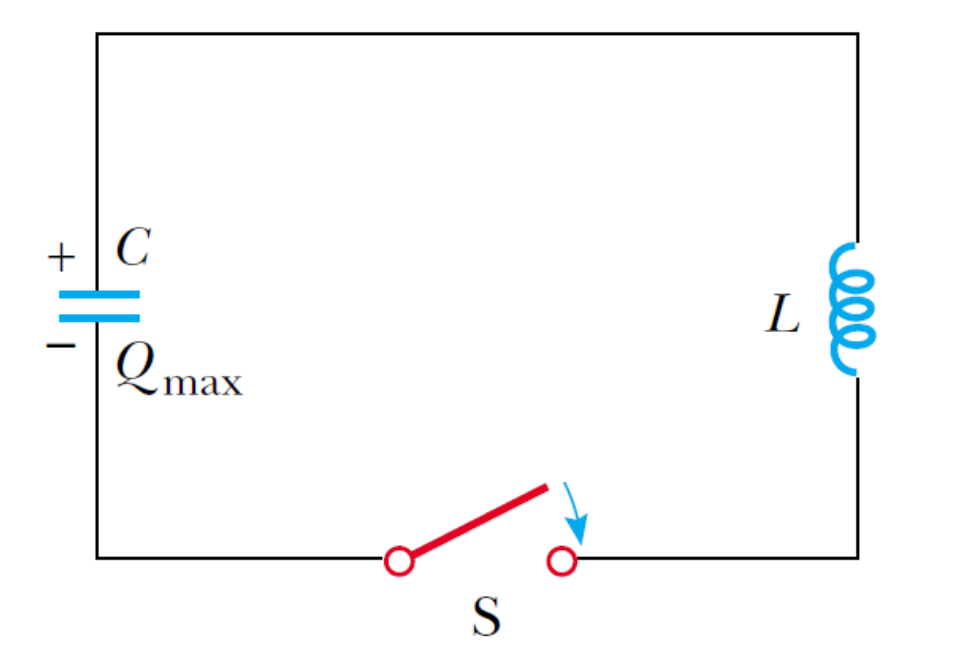
\includegraphics[scale = 0.275]{oz08/resources/Oz8Oef3.png}
\end{minipage}

% \begin{center}
%     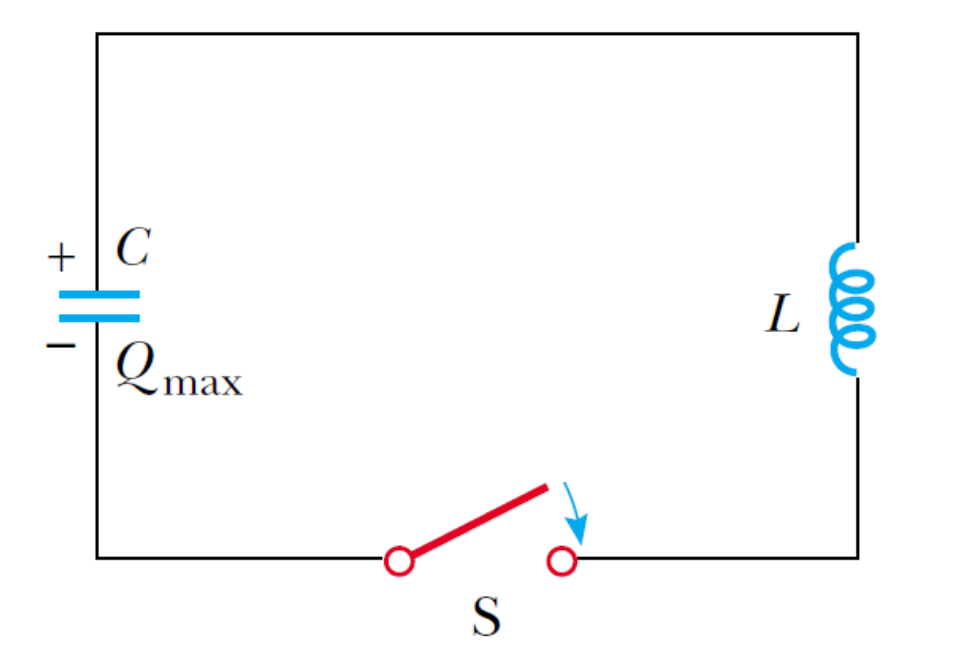
\includegraphics[scale = 0.3]{oz08/resources/Oz8Oef3.png}
% \end{center}

\begin{description}[labelwidth=1.5cm, leftmargin=!]
    \item[Geg. :]   $L = 82.0 \ \text{mH}$, $C = 17.0 \ \mu \text{F}$, $Q_0 = 180 \ \mu \text{C}$
\end{description}

\begin{enumerate}[(a)]
    \item 
        \begin{description}[labelwidth=1.5cm, leftmargin=!]
            \item[Gevr. :] $f$ ?
            \item[Opl. :]   
                Bij een LC-kring is de frequentie van de oscillaties gelijk aan
                \begin{equation*}
                    f = \frac{1}{2\pi\sqrt{LC}} \approx 135 \ \text{Hz}.
                \end{equation*}
        \end{description}
    \item 
        \begin{description}[labelwidth=1.5cm, leftmargin=!]
            \item[Geg. :] $t_1 = 1.00 \ \text{ms}$
            \item[Gevr. :] $Q_1$ ?
            \item[Opl. :]   
                De lading op de condensator in een LC-kring heeft de volgende formule
                \begin{equation*}
                    Q(t) = Q_{\text{max}} \cos(\omega t)
                \end{equation*}
                waarbij $\omega = 2\pi f$. We kunnen nu de lading op de condensator berekenen op $t_1$:
                \begin{equation*}
                    Q_1 = Q_{\text{max}} \cos(\omega t_1) \approx 119 \ \mu \text{C}.
                \end{equation*}
        \end{description}
    \item
        \begin{description}[labelwidth=1.5cm, leftmargin=!]
            \item[Geg. :] $t = 1.00 \ \text{ms}$
            \item[Gevr. :] $I_1$ ?
            \item[Opl. :] 
                De stroom in een LC-kring heeft de volgende formule 
                \begin{equation*}
                    I(t) = I_{\text{max}} \sin(\omega t) = \frac{Q_{\text{max}}}{\sqrt{LC}} \sin(\omega t).
                \end{equation*}
                waarbij $\omega = 2\pi f$. We kunnen nu de stroom berekenen op $t_1$:
                \begin{equation*}
                    I_1 = \frac{Q_{\text{max}}}{\sqrt{LC}} \sin(\omega t_1) \approx 114 \ \text{mA}.
                \end{equation*}
                \textbf{Opmerking:} we hebben hier stroom gezien als 
                \begin{equation*}
                    I(t) = -\frac{dQ}{dt},
                \end{equation*} 
                omdat deze veroorzaakt wordt door het ontladen van de condensator.
        \end{description}
\end{enumerate}


\vspace{1cm}